Pour une sécurité optimale, il est judicieux d'ajouter, en plus des protections mécaniques, des capteurs afin de détecter si une protection est ouverte.

Afin de renforcer la sécurité, un arrêt d'urgence ainsi qu'une clé de maintenance sont ajoutés. Ces deux capteurs sont reliés et connectés à l'interlock du driver du laser.

\section{Interlock: Principe de fonctionnement}

\begin{minipage}[c]{0.6\textwidth}
    Le driver du laser intègre un système d'interlock permettant de désactiver, si le circuit électrique interlock est ouvert, l'alimentation du laser. Par défaut, un pont est soudé entre les pins 1 et 5 (Figure~\ref{No_interlock}).
\end{minipage}\hfill
\begin{minipage}[c]{0.35\textwidth}
    \begin{figure}[H]
        \begin{center}
            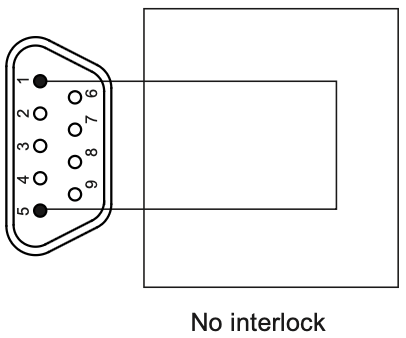
\includegraphics[width=0.8\textwidth]{assets/figures/Protections_laser/Securite_electrique/no_interlock.png}
        \end{center}
        \captionof{figure}{Schéma électrique sans interlock~\cite{LaserDriverKLD101}}
        \label{No_interlock}
    \end{figure}
\end{minipage}
\begin{minipage}[c]{0.6\textwidth}
    L'objectif est d'ajouter un circuit électrique personalisé qui intègre l'interlock. De ce fait, le schéma suivant est utilisé pour la conception du circuit électrique (Figure~\ref{Interlock_only}).
\end{minipage}\hfill
\begin{minipage}[c]{0.35\textwidth}
    \begin{figure}[H]
        \begin{center}
            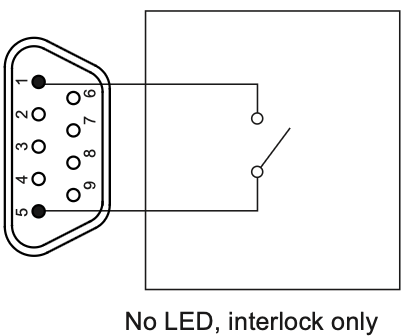
\includegraphics[width=0.8\textwidth]{assets/figures/Protections_laser/Securite_electrique/interlock_only.png}
        \end{center}
        \captionof{figure}{Schéma électrique avec interlock~\cite{LaserDriverKLD101}}
        \label{Interlock_only}
    \end{figure}
\end{minipage}

\newpage
\section{Première version du schéma électrique de l'interlock}
La Figure~\ref{schema_interlock_v1} montre la première version du schéma électrique complet de l'interlock. Comme le choix des capteurs n'est pas encore fait à ce jour, des fins de course ont été représentés de façon provisoire, afin d'avoir une première représentation fonctionnelle du système. L'arrêt d'urgence ainsi que la clé de maintenance seront expliqués à la section~\ref{subsec:arret_urgence_maintenance}.

\begin{figure}[H]
    \begin{center}
        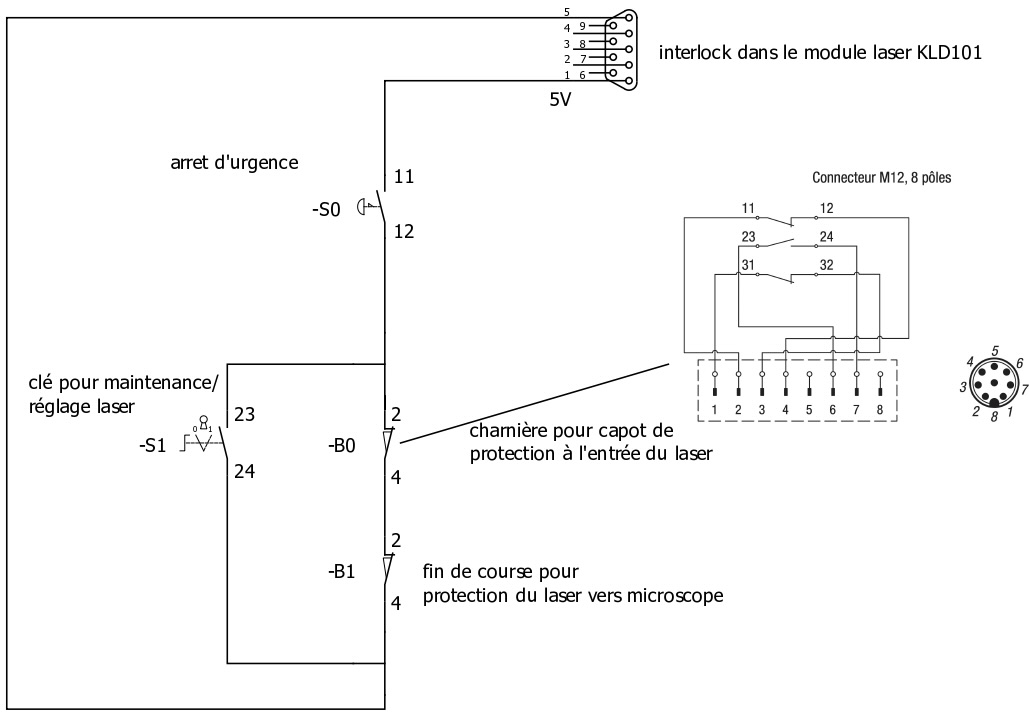
\includegraphics[width=\textwidth]{assets/figures/Protections_laser/Securite_electrique/interlock_schema_elec_V1.jpeg}
    \end{center}
    \caption{Première version du schéma électrique complet de l'interlock}
    \label{schema_interlock_v1}
\end{figure}
\newpage
\section{Capteurs sur les protections mécaniques}
Afin de garantir la sécurité lors de l'utilisation du laser, il est essentiel d'être averti si l'une des deux protections est ouverte.

\subsection{Solutions disponibles sur le marché}
\begin{minipage}[c]{0.6\textwidth}
    % Une première recherche s'est portée sur des interrupteurs de sécurité avec vérouillage électrique, que l'on retrouve beaucoup dans l'industrie. Ci-contre, un exemple de ce type d'interrupteur (Figure~\ref{interrupteur_telemecanique}).

    Ces serrures ont l'avantage d'être vérouillées électriquement, ce qui permet d'assurer un vérouillage mécanique. Malheureusement, ce type de sécurité est trop volumineux pour notre système.
\end{minipage}\hfill
\begin{minipage}[c]{0.35\textwidth}
    \begin{center}
        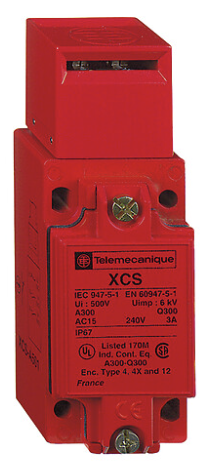
\includegraphics[width=0.45\textwidth]{assets/figures/Protections_laser/Securite_electrique/serrure_telemecanique.png}
    \end{center}
    \captionof{figure}{Interrupteur de sécurité Telemecanique~\cite{interrupteurTelemecanique}}
    \label{interrupteur_telemecanique}
\end{minipage}

\begin{minipage}[c]{0.6\textwidth}
    Le constructeur d'organes de sécurité Pilz propose une charnière comprenant un capteur intégré, qui permet de régler librement le point de commutation du contact entre 0\textdegree{} et 270\textdegree{}.

    % La Figure~\ref{charniere_pilz} montre un exemple de ce type de charnière électrique.
\end{minipage}\hfill
\begin{minipage}[c]{0.35\textwidth}
    \begin{center}
        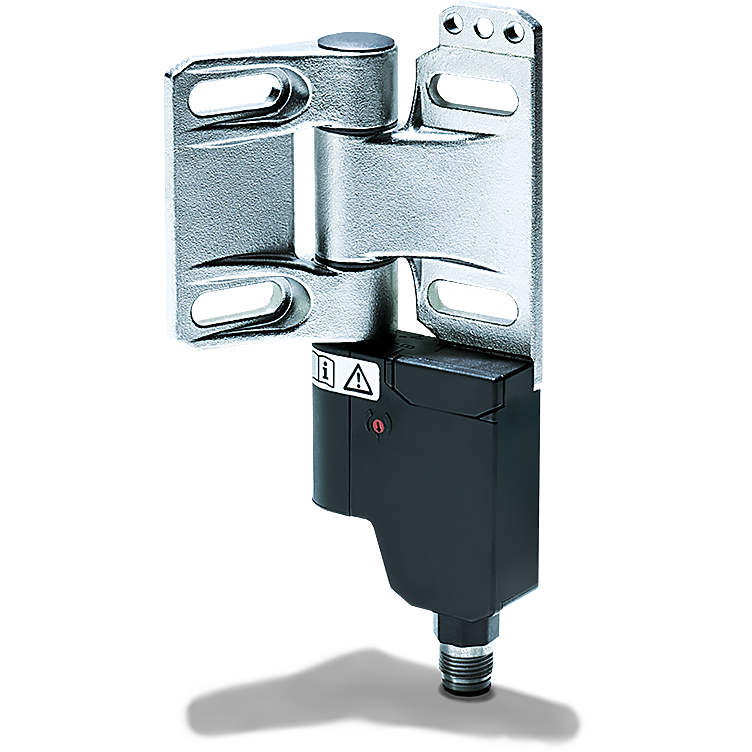
\includegraphics[width=0.6\textwidth]{assets/figures/Protections_laser/Securite_electrique/charniere_pilz.png}
    \end{center}
    \captionof{figure}{Charnière de sécurité Pilz~\cite{charnierePilz}}
    \label{charniere_pilz}
\end{minipage}

\begin{minipage}[c]{0.6\textwidth}
    Une dernière option de charnière de sécurité a été élaborée par l'entreprise Norelem. Avec cette charnière, on peut également régler l'angle de commutation. L'avantage de celle-ci est que le capteur est directement intégré dans la charnière, le rendant totalement invisible.

    % La Figure~\ref{charniere_norelem} montre la charnière de Norelem.
\end{minipage}\hfill
\begin{minipage}[c]{0.35\textwidth}
    \begin{center}
        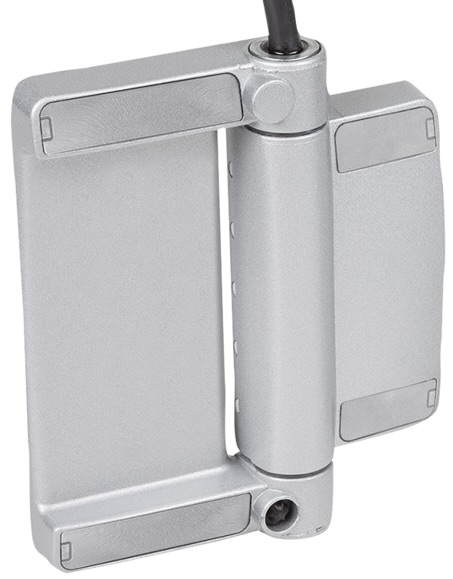
\includegraphics[width=0.75\textwidth]{assets/figures/Protections_laser/Securite_electrique/charniere_norelem.jpeg}
    \end{center}
    \captionof{figure}{Charnière de sécurité Norelem~\cite{charniereNorelem}}
    \label{charniere_norelem}
\end{minipage}

\begin{minipage}[c]{0.6\textwidth}
    Le fin de course est souvent utilisé en électronique, car il ne prend pas beaucoup de place et il est facile à implémenter. Bien que cette solution soit discrète, cela reste un système de sécurité simple, et peut être facilement contourné.

    % La Figure~\ref{fin_de_course} montre un fin de course.
\end{minipage}\hfill
\begin{minipage}[c]{0.35\textwidth}
    \begin{center}
        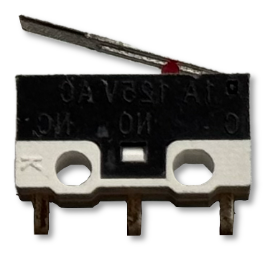
\includegraphics[width=0.6\textwidth]{assets/figures/Protections_laser/Securite_electrique/fin_de_course.png}
    \end{center}
    \captionof{figure}{Fin de course}
    \label{fin_de_course}
\end{minipage}

\newpage
\subsection{Solution choisie pour la protection à l'entrée du laser}
La solution finale pour cette protection s'est tournée sur la charnière de sécurité de l'entreprise Norelem. Elle contient tous les avantages que l'on recherche pour ce travail, notamment :
\begin{itemize}[label=\textbullet]
    \item Elle s'intègre dans la conception de la protection, car il est nécessaire d'avoir une charnière pour soulever celle-ci.
    \item Elle contient un capteur de position intégré.
    \item L'angle de commutation est réglable.
    \item Elle est compacte, ce qui facilite son intégration dans le kit actuel.
    \item Il s'agit d'une solution robuste, conçue pour un usage industriel, ce qui assurera son efficacité dans le temps.
\end{itemize}

\subsection{Solution choisie pour la protection vers le microscope}
La solution finale pour cette protection s'est tournée sur le fin de course. Ses principaux avantages sont  :
\begin{itemize}[label=\textbullet]
    \item Il n'y a pas beaucoup de place vers le microscope pour faire une protection, par conséquent, sa taille permet d'être installée presque où l'on souhaite.
    \item Il est peu coûteux et facilement remplaçable.
    \item Malgré sa sécurité simple, des solutions existent pour cacher le fin de course afin qu'il ne soit pas accessible facilement.
\end{itemize}

\section{Boîtier de sécurité : arrêt d'urgence et clé de maintenance}
\label{subsec:arret_urgence_maintenance}
L'ajout d'un arrêt d'urgence est l'une des principales sécurité électrique que l'on retrouve sur tout type de système électrique. Comme indiqué sur le schéma électrique de la Figure~\ref{schema_interlock_v1}, l'arrêt d'urgence est en série de tout le circuit interlock, ce qui permet de couper l'alimentation du laser à tout moment en pressant dessus.

La clé de maintenance est câblée en parallèle des deux capteurs. Comme son nom l'indique, enclencher cette clé, permet de faire la maintenance. En effet, dans cette position le contact est fermé, ce qui permet aux deux capteurs de ne plus avoir d'influence sur l'ouverture du circuit interlock. Il peut arriver de devoir effectuer des réglages sur les lentilles réglables ou sur le laser. Dans ce cas, le laser doit rester allumé même avec les protections ouvertes (Figure \ref{boitier_arret_urgence_maintenance}).

\begin{figure}[H]
    \begin{center}
        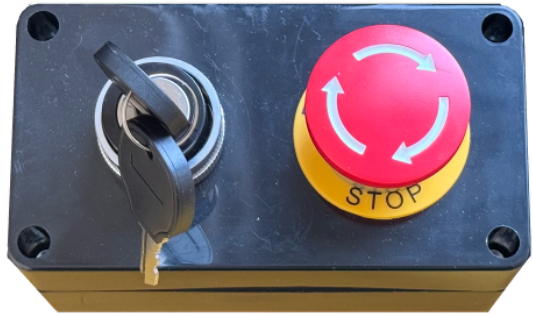
\includegraphics[width=0.5\textwidth]{assets/figures/Protections_laser/Securite_electrique/boitier_arret_urgence_maintenance.png}
    \end{center}
    \caption{Boîtier comprenant l'arrêt d'urgence et la clé de maintenance}
    \label{boitier_arret_urgence_maintenance}
\end{figure}

\section{Version finale du schéma électrique de l'interlock}
Une fois les capteurs choisis, le schéma électrique est remis à jour. Le changement a été fait au niveau des noms de bornes, afin qu'ils correspondent aux noms indiqués sur chaque capteur.

\begin{figure}[H]
    \begin{center}
        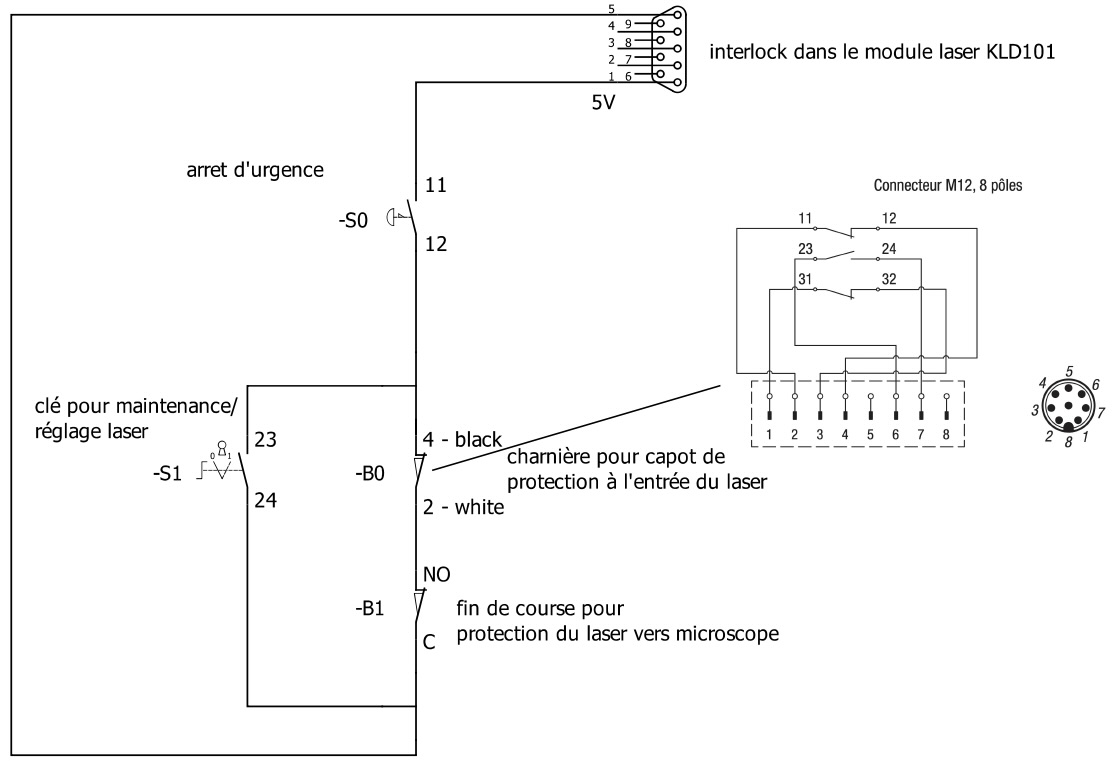
\includegraphics[width=\textwidth]{assets/figures/Protections_laser/Securite_electrique/interlock_schema_elec_V2.jpg}
    \end{center}
    \caption{Version finale du schéma électrique complet de l'interlock}
    \label{schema_interlock_v2}
\end{figure}
\newpage
\section{Câblage de l'interlock}
\begin{minipage}[c]{0.48\textwidth}
    Une fois tous les composants en place, le câblage de l'interlock est exécuté. La Figure~\ref{cablage_vers_connecteur_laser} montre le fil rouge et le fil noir qui sortent du connecteur du laser et sont utilisés pour le circuit de l'interlock.
\end{minipage}\hfill
\begin{minipage}[c]{0.48\textwidth}
    \begin{center}
        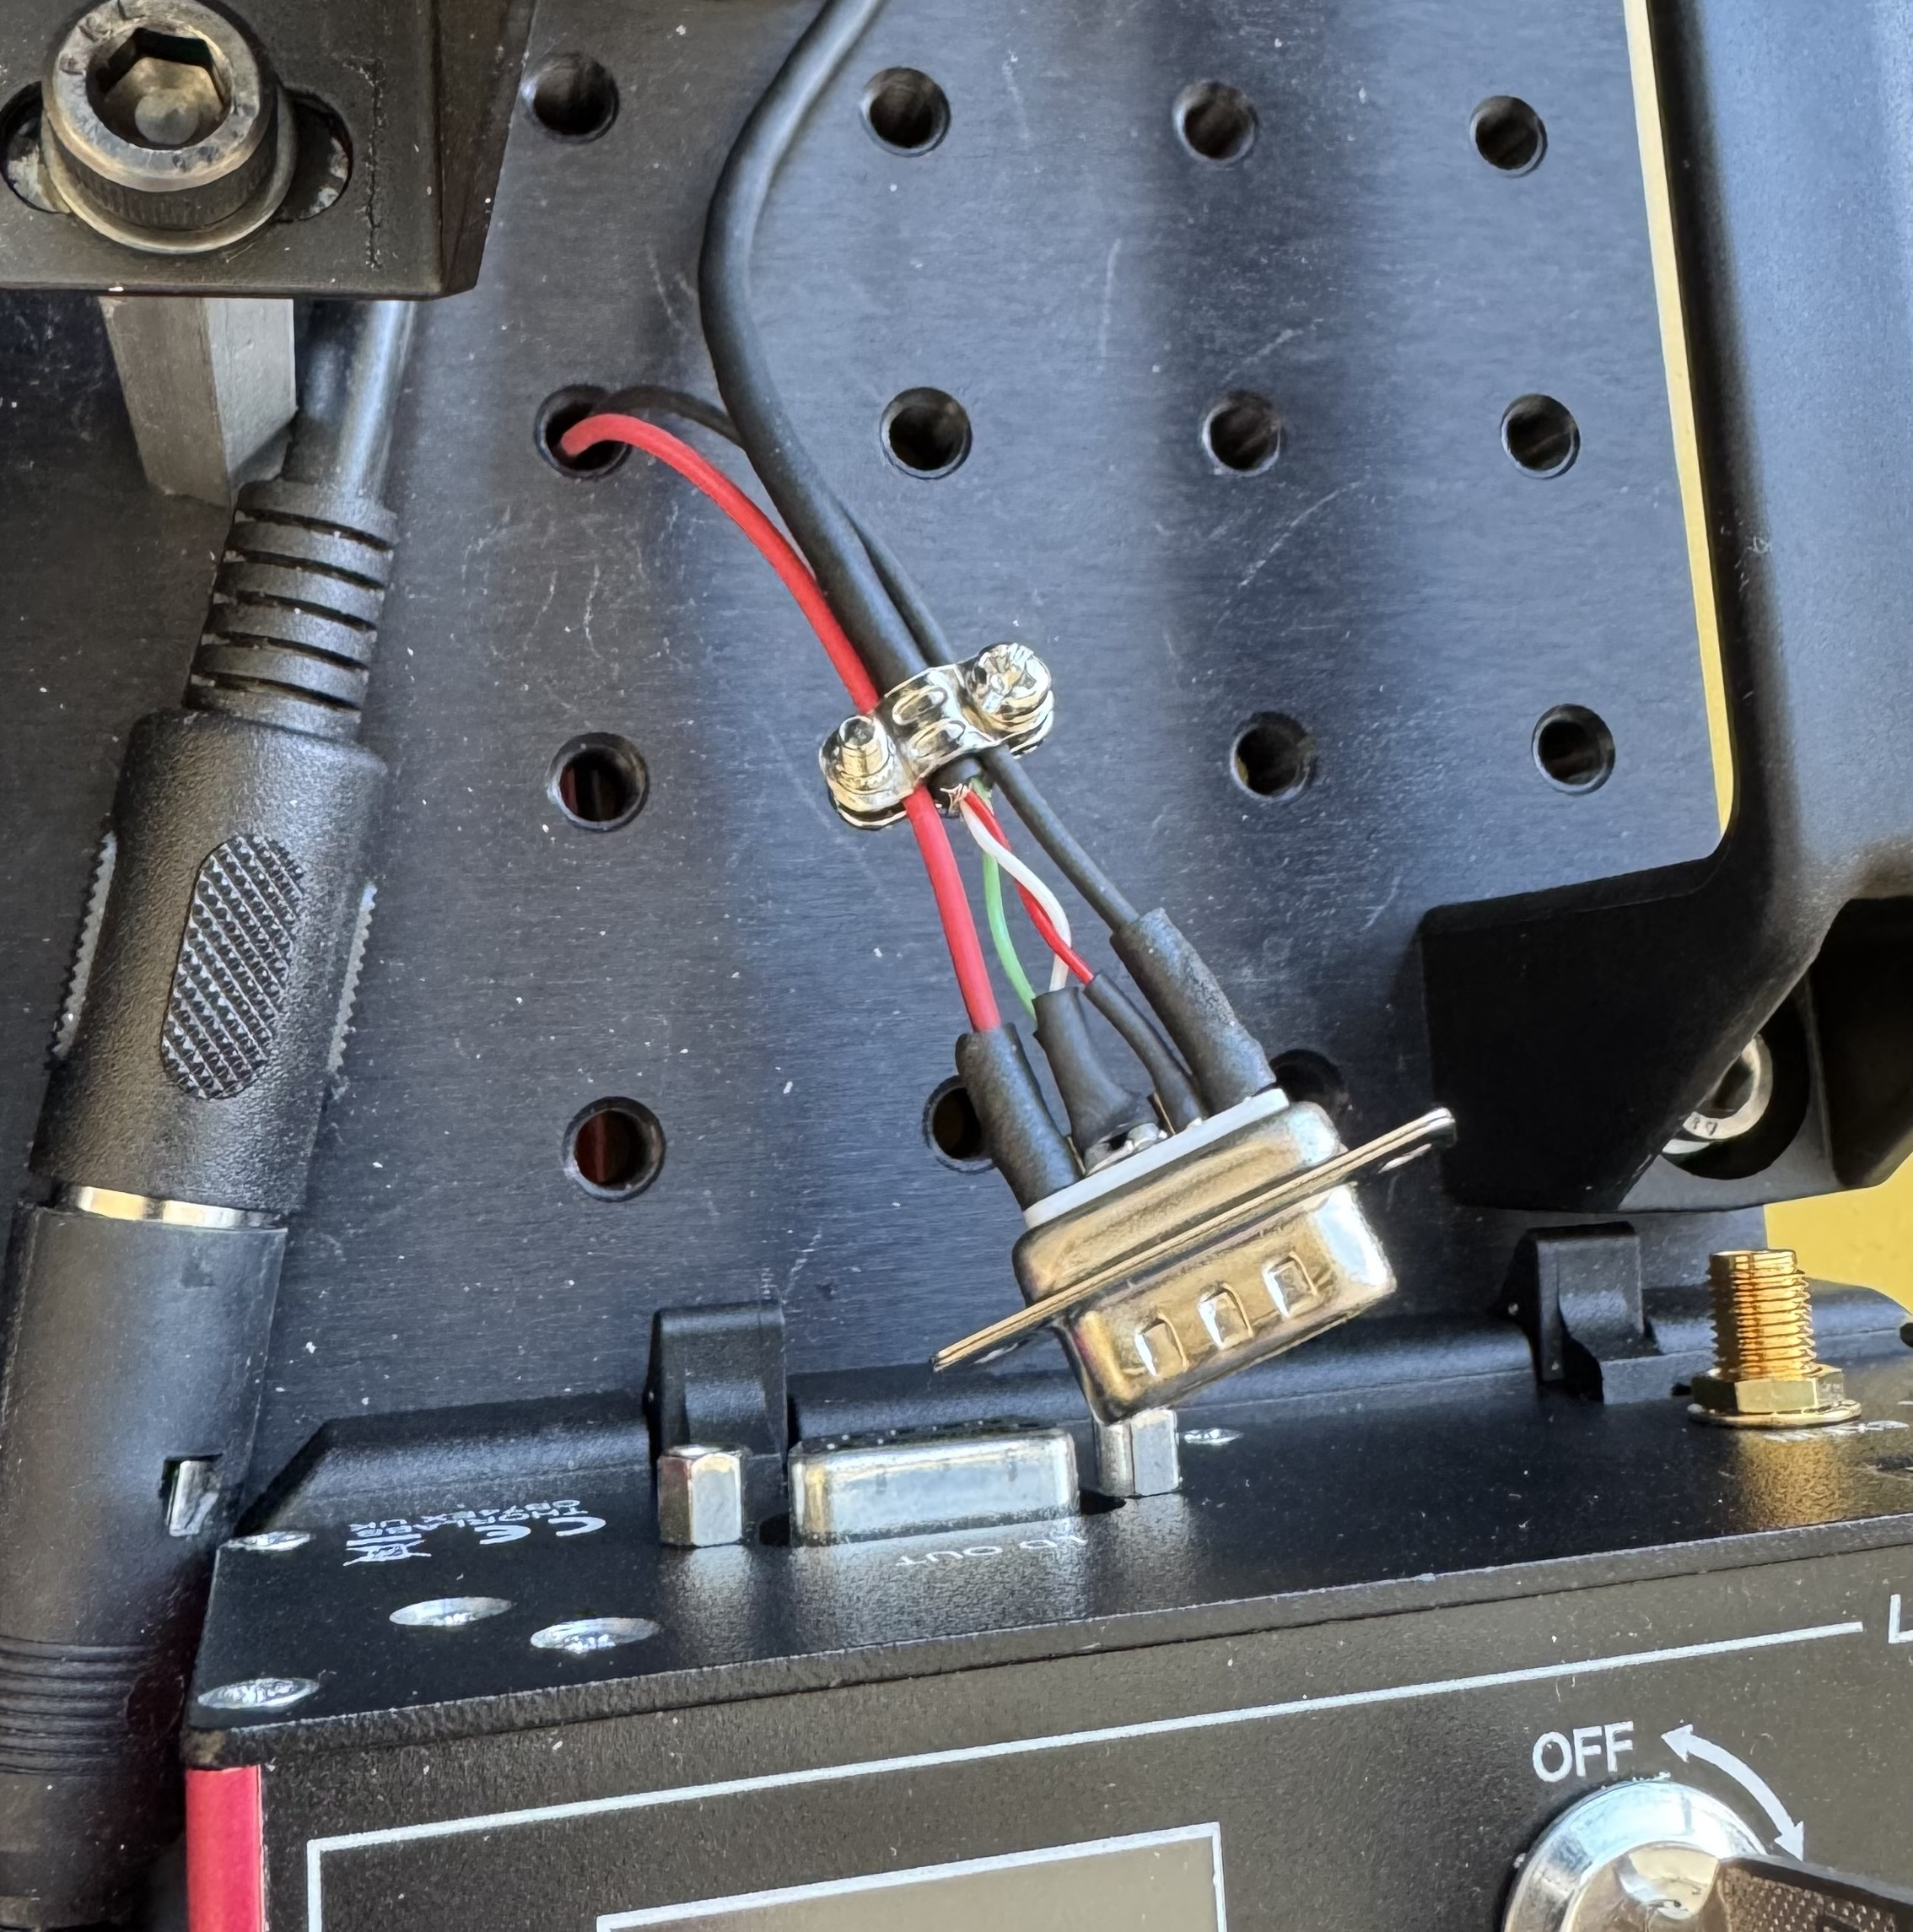
\includegraphics[width=0.9\textwidth]{assets/figures/Protections_laser/Securite_electrique/cablage_vers_connecteur_laser.jpeg}
    \end{center}
    \captionof{figure}{Connexion des deux fils, rouge et noir, sortant du connecteur du laser}
    \label{cablage_vers_connecteur_laser}
\end{minipage}

\begin{minipage}[c]{0.48\textwidth}
    Comme montré sur la Figure~\ref{cablage_sous_plaque_de_montage}, ces fils passent sous la plaque de montage en aluminium et rejoignent le boîtier contenant l'arrêt d'urgence et la clé de maintenance. Ceux-ci sont indiqués par la flèche \textcolor[RGB]{115, 210, 210}{bleue}.

    \vspace{1em}
    La flèche \textcolor{red}{rouge}, montre les deux fils reliant le contact normalement ouvert dans le fin de course. Eux aussi rejoignent le boîtier par dessous.
\end{minipage}\hfill
\begin{minipage}[c]{0.48\textwidth}
    \begin{center}
        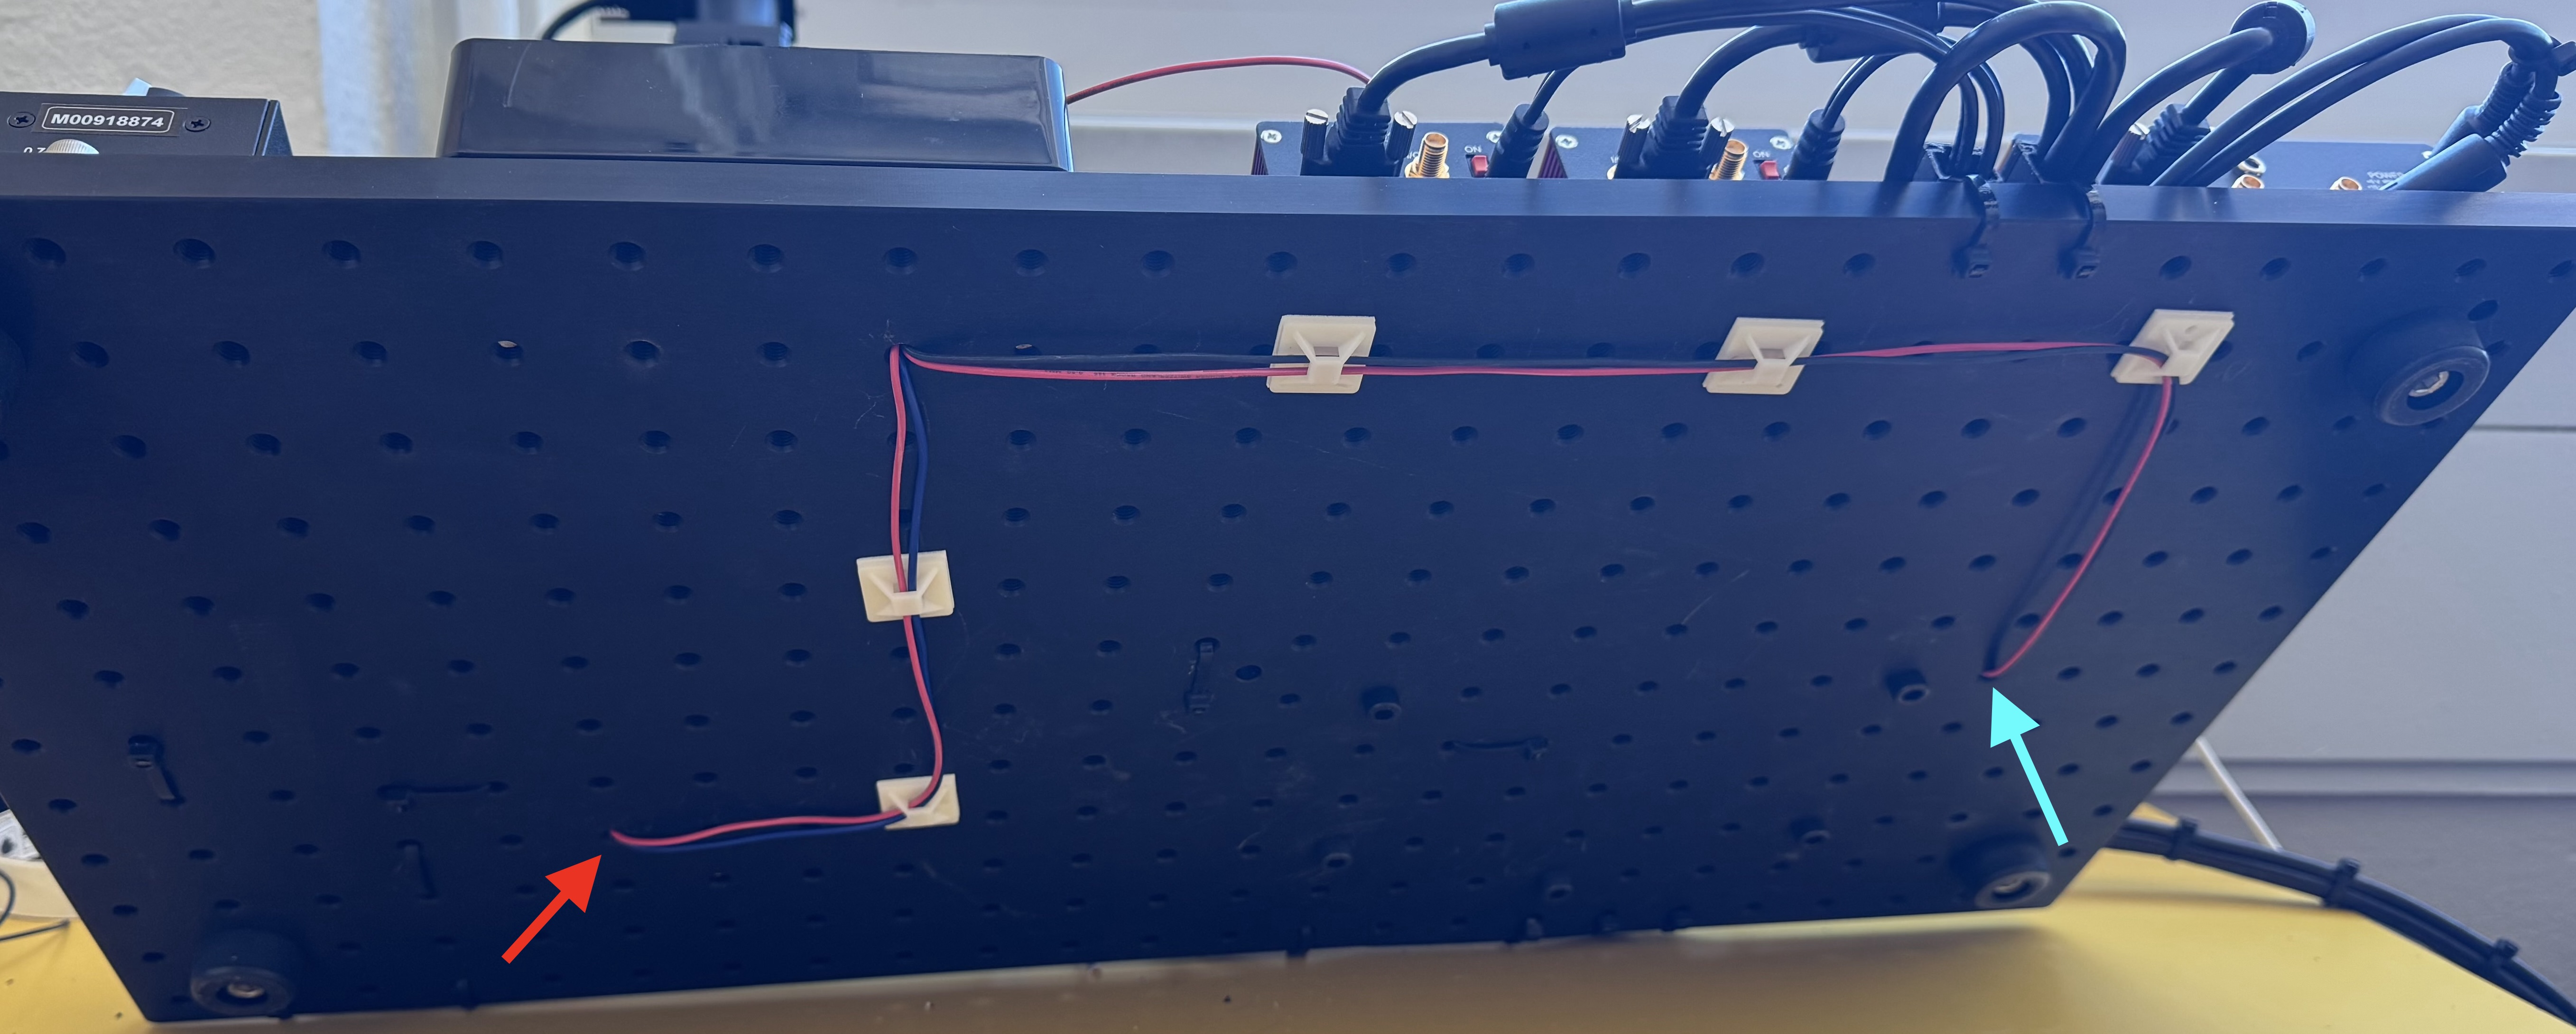
\includegraphics[width=\textwidth]{assets/figures/Protections_laser/Securite_electrique/cablage_sous_plaque_de_montage.jpeg}
    \end{center}
    \captionof{figure}{Passage des deux fils de l'interlock sous la plaque de montage en aluminium}
    \label{cablage_sous_plaque_de_montage}
\end{minipage}

\begin{minipage}[c]{0.48\textwidth}
    Finalement, en suivant le schéma électrique (Figure~\ref{schema_interlock_v2}), tous les composants de sécurité se retrouvent dans le boîtier afin d'être connecté ensemble, comme illustré sur la Figure~\ref{cablage_dans_boitier}.
\end{minipage}\hfill
\begin{minipage}[c]{0.48\textwidth}
    \begin{center}
        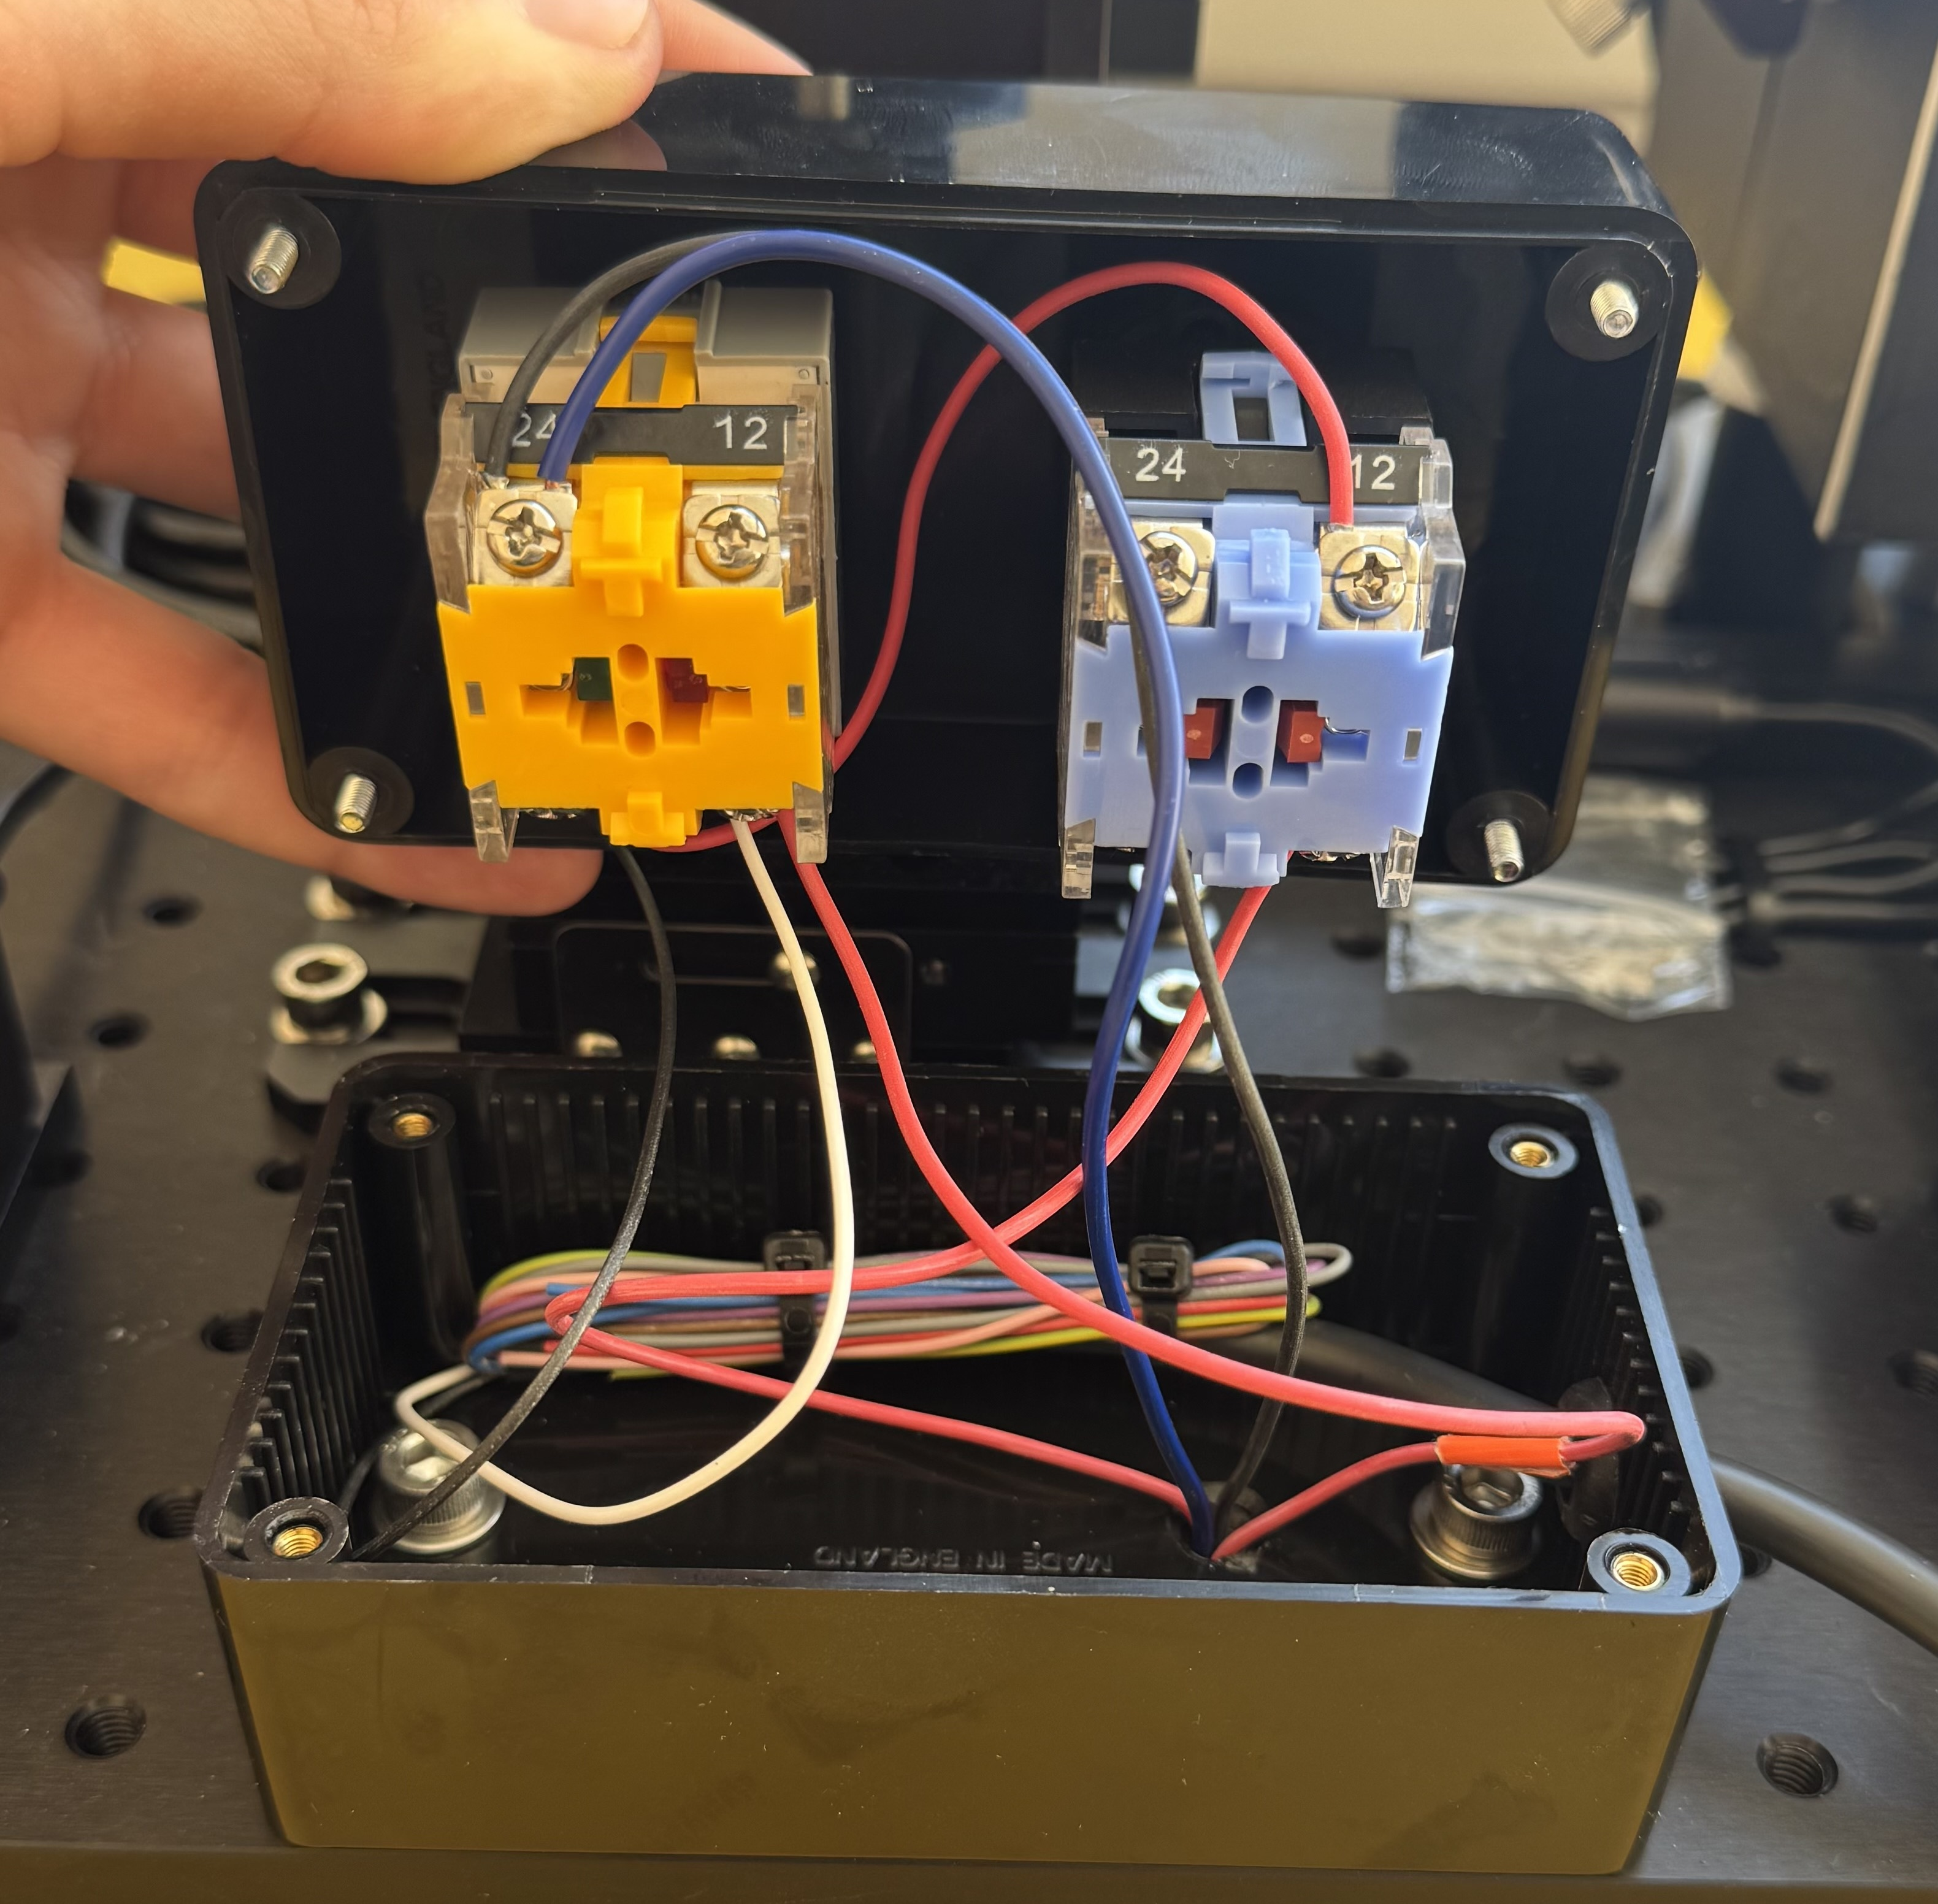
\includegraphics[width=\textwidth]{assets/figures/Protections_laser/Securite_electrique/cablage_dans_boitier.jpeg}
    \end{center}
    \captionof{figure}{Câblage des composants de sécurité dans le boîtier}
    \label{cablage_dans_boitier}
\end{minipage}

\section{Maintenance}

\begin{minipage}[c]{0.48\textwidth}
    La maintenance permet de pouvoir régler les différents composants du système. Pour assurer la sécurité lors de cette action, il est \textbf{obligatoire} d'utiliser des lunettes de sécurité adaptées contre les lasers. La Figure~\ref{lunettes_securite} montre les types de lunettes misent à disposition.
\end{minipage}\hfill
\begin{minipage}[c]{0.48\textwidth}
    \begin{center}
        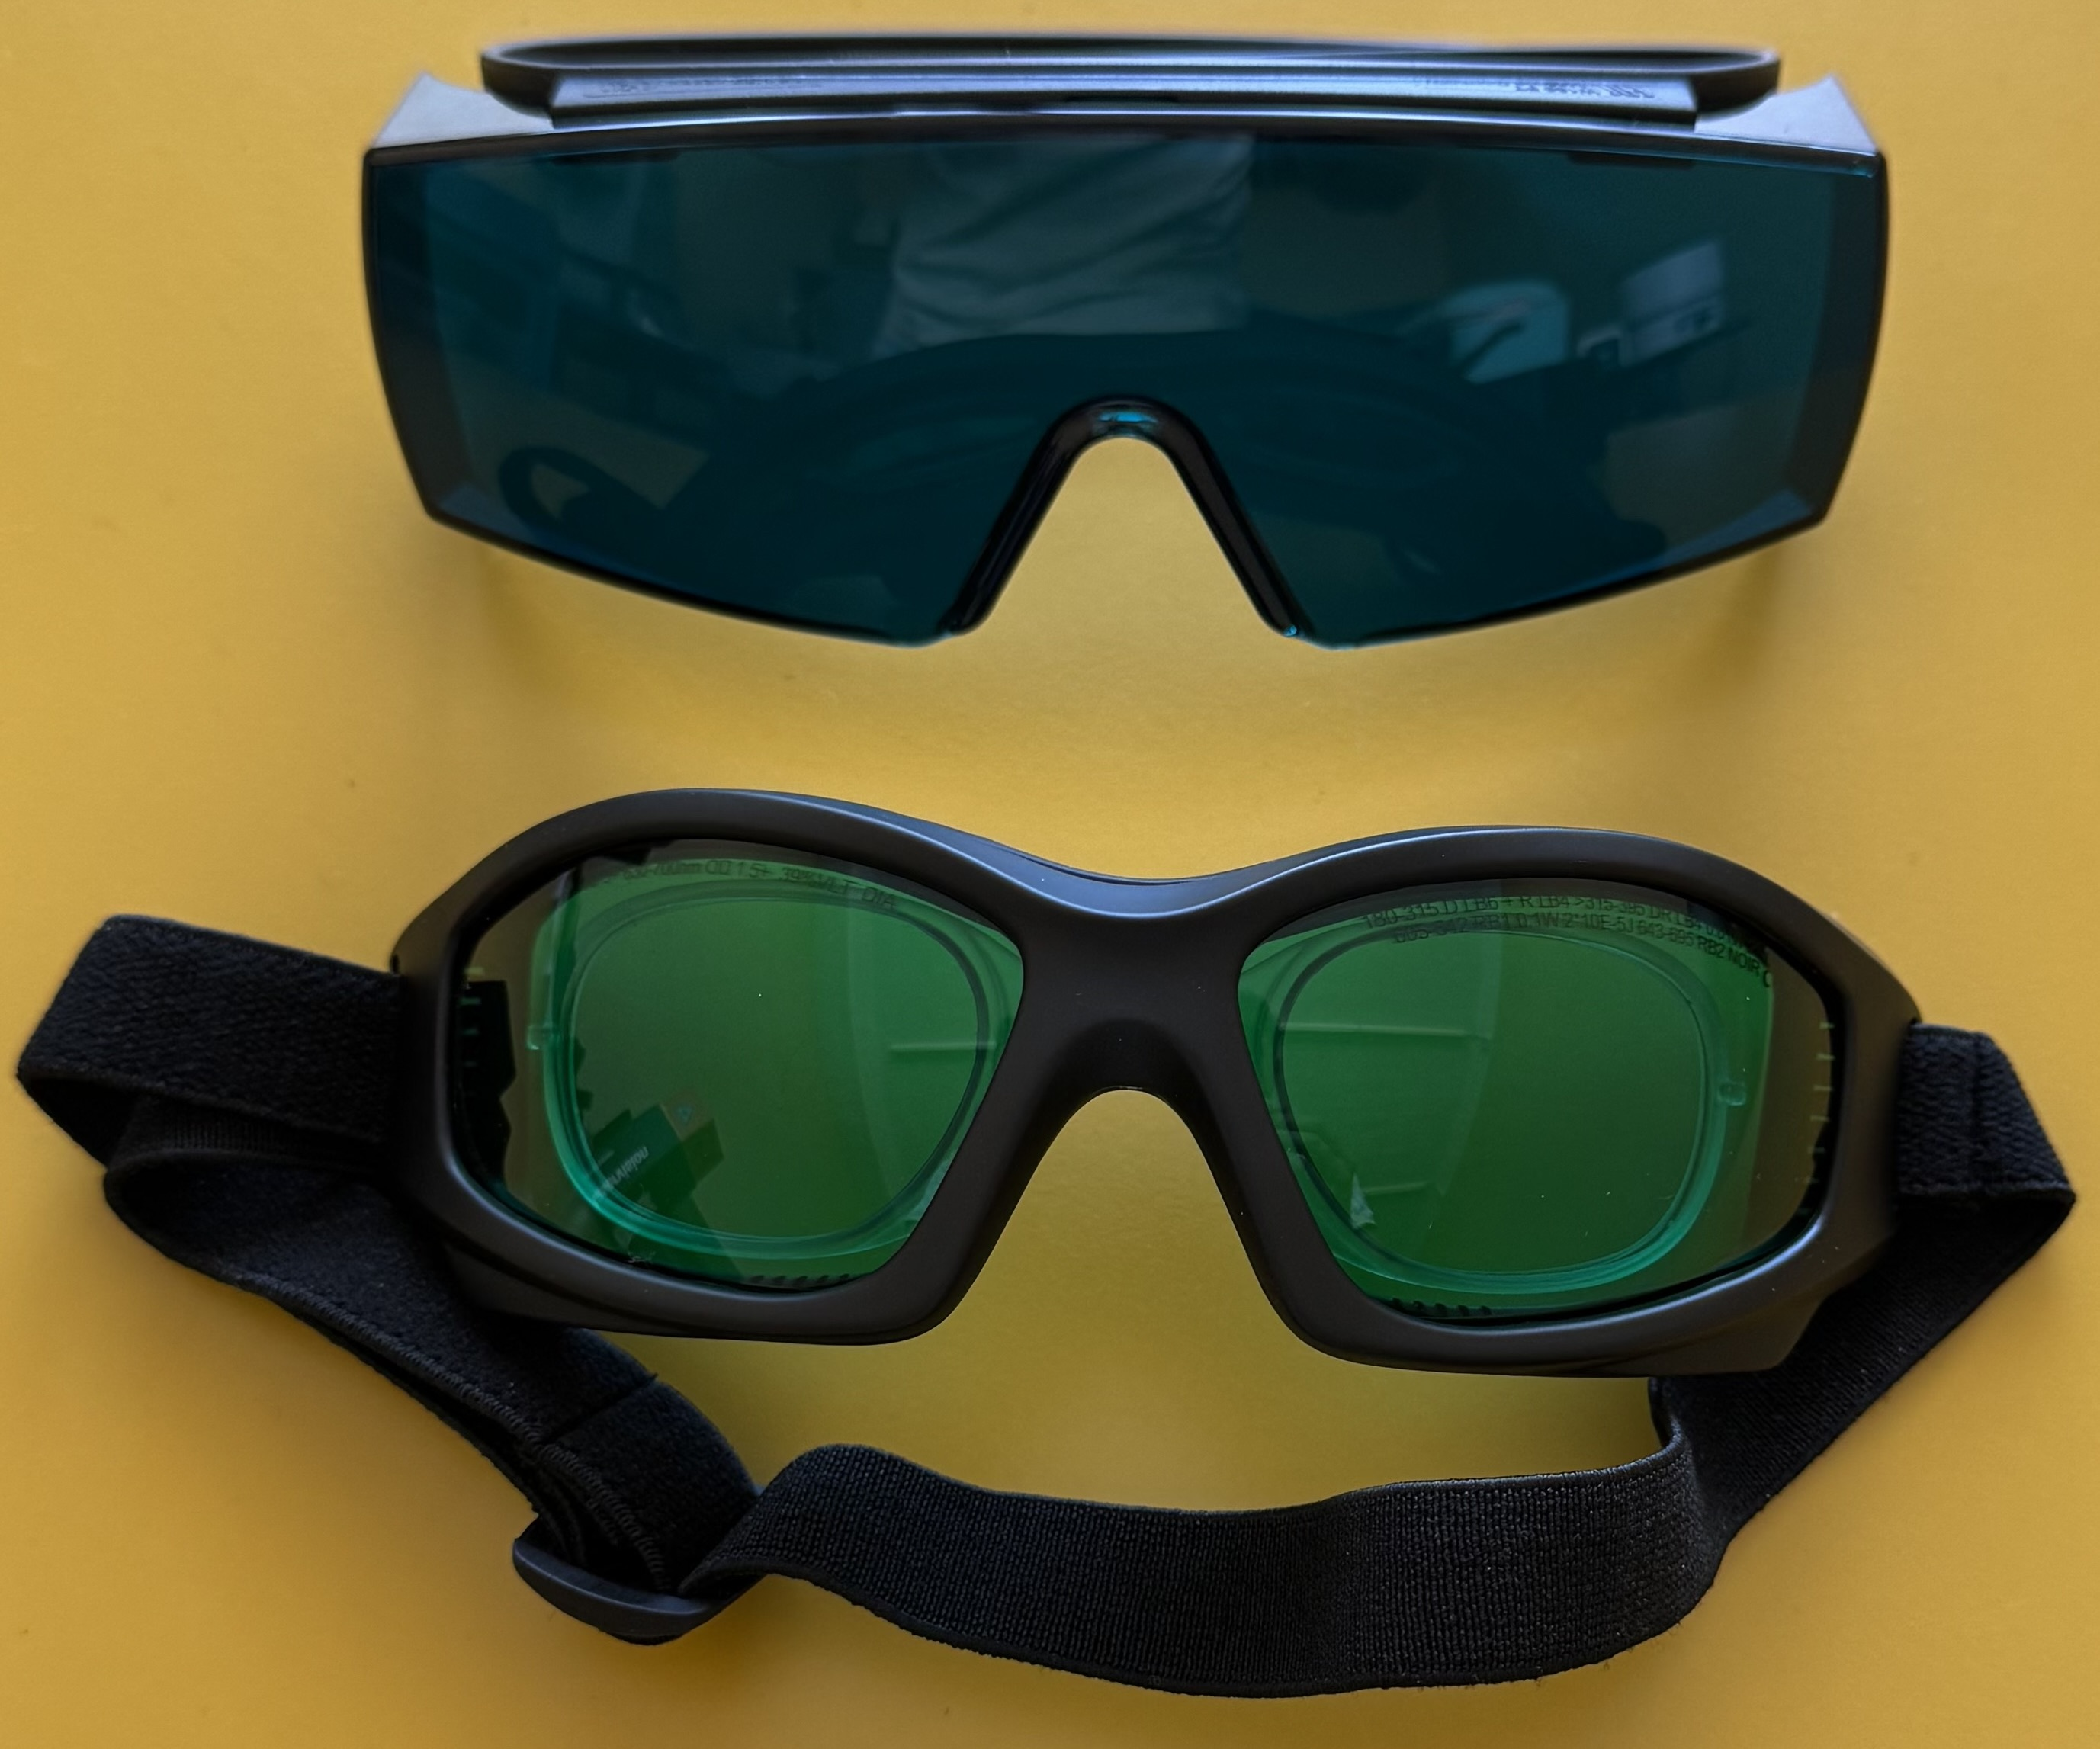
\includegraphics[width=0.8\textwidth]{assets/figures/Protections_laser/Securite_electrique/lunettes_securite.jpeg}
    \end{center}
    \captionof{figure}{Lunettes de sécurité disponibles avec le système pour la maintenance}
    \label{lunettes_securite}
\end{minipage}